% .:: Laden der LaTeX4EI Formelsammlungsvorlage
\documentclass[fs, footer]{latex4ei}

% Dokumentbeginn
% ======================================================================
\begin{document}

% .:: Aufteilung in Spalten
\vspace{-4mm}
\begin{multicols*}{4}

% .:: LOGO ================================================================
	\fstitle{Elektronische \\ Bauelemente}
% =========================================================================


% -------------------------------------------
% | 		Elektronische Bauelemente		|
% ~~~~~~~~~~~~~~~~~~~~~~~~~~~~~~~~~~~~~~~~~~~

% .:: SECTION =============================================================
\section{Grundlagen}
% =========================================================================
\sectionbox{

	\subsection{Masse, Dichte, Stoffmenge}
	Masse $m_x = V_x \cdot \rho_x = V_x \cdot n_x \cdot m_{\ir A}$\\
	Stoffmenge $n_{\ir mol} = \frac{N}{N_{\ir A}} = \frac{m}{m_{\ir A}}$\\


	\subsection{Eigenschaften von Halbleiterng}
	Widerstand: $R = \rho \frac{l}{A}$

	\subsection{Intrinsische Halbleiter (Eigenleitend)}
	\tablebox{
	\begin{tabular*}{\columnwidth}{@{\extracolsep\fill}ll@{}}
	\ctrule
	\textbf{Leitungsband} & \textbf{Valenzband}\\ \cmrule
	Elektronendichte & Löcherdichte\\
	$n = \int\limits_{E_{\ir L}}^\infty D_{\ir L} \cdot f_e \diff E$ & $p = \int\limits_{-\infty}^{E_{\ir V}} D_{\ir V} \cdot f_h \diff E$\\[2em]
	Zustandsdichte  & Zustandsdichte\\
	$D_{\ir L} = \frac{(2 m_n^*)^{3/2}}{2 \pi^2 \hbar^3} \sqrt{E-E_{\ir L}}$ & $D_{\ir V} = \frac{(2 m_p^*)^{3/2}}{2 \pi^2 \hbar^3} \sqrt{E_{\ir V} - E}$\\[2em]
	Effektive Zustandsdichte & Effektive Zustandsdichte\\	
	$N^*_{\ir L} = 2 \left( \frac{m_n^* k_{\ir B} T}{2 \pi \hbar^2}\right)^{3/2}$ & $N^*_{\ir V} = 2 \left( \frac{m_p^* k_{\ir B} T}{2 \pi \hbar^2}\right)^{3/2}$\\
	$n = N^*_{\ir L} \exp\left(-\frac{E_{\ir L} - E_{\ir F}}{k_{\ir B}\cdot T}\right)$ & $p = N^*_{\ir V} \exp\left(-\frac{E_{\ir F} - E_{\ir V}}{k_{\ir B}\cdot T}\right)$ \\ 
	\cbrule
	\end{tabular*}
	}	
	
	
	
	\subsection{Dotierung von Halbleitern}		

	% Bild von Bändermodell mit Donatoren/Akzeptoren
	\tablebox{
	\begin{tabular*}{\columnwidth}{l@{\extracolsep\fill}l} \ctrule
	{\large \textbf{n}}-Dotierung $+1e^-$ & {\large \textbf{p}}-Dotierung $+1h^+$\\ \cmrule
	Donator aus \rom{V} & Akzeptor aus \rom{III}\\
	$N_{\ir D} = N_{\ir D}^0 + N_{\ir D}^+$ & $N_{\ir A} = N_{\ir A}^0 + N_{\ir A}^+$\\
	$N_{\ir A} = 0$ & $N_{\ir D} = 0$\\[1em]
	%$n \approx N_{\ir D}^+$ & $p \approx N_{\ir A}^-$\\ siehe Tempnäherung
	$N_{\ir D}^{0} = N_{\ir D} \cdot f(E_{\ir D},T)$ & $N_{\ir A}^0 = N_{\ir A} [1 - f(E_{\ir A},T)]$\\ 	
	$N_{\ir D}^+ = N_{\ir D} [ 1- f(E_{\ir D},T)]$ & $N_{\ir A}^{-} = N_{\ir A} \cdot f(E_{\ir A},T)$\\ [1em]
	Bei Raumtemp. und $N_{\ir D} \gg n_{\ir i}$ & Bei Raumtemp. und $N_{\ir A} \gg n_{\ir i}$\\
	$n \approx N_{\ir D}^+ \approx N_{\ir D}$ & $p \approx N_{\ir D}^+ \approx N_{\ir D}$ \\[1em]
	$E_{\ir F,n} = E_{\ir L} - k_{\ir B} T \ln \frac{N_{\ir C}}{N_{\ir D}^+}$ & $E_{\ir F,p} = E_{\ir V} - k_{\ir B} T \ln \frac{N_{\ir V}}{N_{\ir A}^-}$ \\ \cbrule
	
	\end{tabular*} }\\
	Amphoter: Sowohl n- als auch p-Dotierung. Bei \rom{III}-\rom{V} HL: \rom{IV}\\
	\\
	Näherungen:\\
	Majoritätsträgerdichte $= \abs{N_{\ir D} - N_{\ir A}}$\\
	Minoritätsträgerdichte $= \frac{n_i^2}{\abs{N_{\ir D} - N_{\ir A}}}$\\
	\\
	\emphbox{
	$\underset{\text{Falls }|E_{\ir C} - E_{\ir F}| > 4 k_{\ir B} T}{\text{Boltzmann-Näherung:}}$ \hfill $f_e(E,T) \approx \exp\left(-\frac{E-E_F}{k_B T}\right)$\\[0.5em]
	Massenwirkungsgesetz: \hfill $n \cdot p = n^2_{\ir i} = N^*_{\ir L} \cdot N^*_{\ir V} \cdot e^{-\frac{E_{\ir g}}{k_{\ir B} T}} $\\[0.5em]
	Dotierungs-Bilanzgleichung: \hfill $n + N_{\ir A}^{-} = p + N_{\ir D}^{+}$\\[0.5em]
	Leitfähigkeit: \hfill $\sigma = n \cdot e \cdot \mu_n + p \cdot e \cdot \mu_p $\\
	}

	Nettoträgerdichte: $N = N_{\ir D} - N_{\ir A}$\\
	Exakt: Falls $\abs{N} \approx n_{\ir i}$: $n_0 = \frac{N}{2} + \sqrt{\left(\frac{N}{2}\right)^2 + n_{\ir i}^2}$\\
	Ab Dotierung $> 10^{11}$ gilt $n \approx N_{\ir D}^+ \approx N_{\ir D}$\\

	} 

\sectionbox{
	\subsection{Bändermodel}
		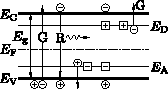
\includegraphics{./img/bandmodel.pdf}


}


\sectionbox{
	\subsection{Halbleitereffekte}
	
	\paragraph{Kombination/Rekombination} von Elektronen und Löchern mit Generationsrate $G$ und Rekombinationsrate $R$.
	Im GGW: $G = R = r(t) n_0 p_0$ 
	
	\paragraph{Lawineneffekt:} Elektrisches Feld beschleunigt elektronen so stark, dass sie beim Zusammenstoß Atome ionisieren.
	Dabei werden elektronen frei, die wiederum beschleunigt werden und Atome ionisieren.

	\paragraph{Eigenleitung:} Nur durch Halbleiter eigene Elektron-Löcher Paare verursachter Ladungstransport.


	\paragraph{Relaxationsprozess} Nach dem das thermodyn. GGW der Ladungsträgerkonzentration gestört wurde, erholt sich Halbleiter.\\
	Überschuss:	$n' = n - n_0$ bzw. $p' = p - p_0$ entspr. Störung, da $n' \ne p'$.\\
	Zeitlich: $p'(t) = p'(0) \cdot \exp\left(-\frac{t}{\tau_{\ir d}} \right)$ \quad $\tau_d = \frac{\varepsilon}{\sigma}$\\
	Räumlich: $p'(x) = p'(0) \cdot \exp\left(-\frac{x}{L_{\ir p}} \right)$ \qquad $L_{\ir p} = \sqrt{D_{\ir p} \tau_{\ir d} }$\\

	\paragraph{Intrinsisch(Undotiert):}
	 $N_{\ir A} = N_{\ir D} = 0$. Eigenleitung durch Generation/Rekombination von Elektron/Loch Paaren über $E_{G}$

	\paragraph{Dotiert:} Störstellenleitung durch Ionisierung/Neutralisierung von Donatoren/Akzeptoren \\
	Anlegen von elektrischem Feld führt zu Bandverbiegung und indirekten Übergängen
	
	\paragraph{Thermospannung: (Seebeck)} Ladungsträger bewegen sich zum kalten Ende.\\
	
	\paragraph{Hall-Effekt:} Lorentzkraft verursacht Querspannung im stromdurchflossenen Leiter $F_{\ir L} = \pm e(v_k \times \vec B)$\\
	$R_{\ir Hn} = \frac{-r}{n \cdot e}$ \\
	$\vec E = \vec E_\parallel + \vec E_\perp = \underbrace{\frac{\vec j_n}{\sigma_n}}_{\vec E_\parallel} \underbrace{- R_n(\vec j_n \times \vec B)}_{\vec E_\perp}$\\
	Elektrisches Feld wirkt Lorentzkraft entgegen: gerader Stromfluss\\
	Kurzschluss: Keine Ladungsträgeranhäufung


	
}


\sectionbox{
	\subsection{Driftströme}
	\emphbox{$\vec v = \mu \vec E$ \qquad für $\norm{\vec E}< \SI{e4}{\volt \per \centi \meter}$ }
	\parbox{2cm}{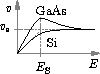
\includegraphics{./img/vE_char.pdf}} \parbox{4cm}{ Sättigugsfeldstärke $\norm{\vec E_S} \approx \SI{e4}{\volt \per \centi \meter}$ \\ Sättigungsgeschwin. $v_s \approx \SI{e7}{\centi \meter \per \second}$}

	$\vec v = \mu(N_{\ir D},T) \cdot \vec E$ \qquad $N_{\ir D} \upa  \Ra \mu \downa \qquad T \upa \Ra \mu \upa$\\

	\begin{tabular}{ll}
	Elektronen & Löcher \\
	$i_n = e\cdot D_n \frac{\partial n}{\partial x}$ & $i_p = - e\cdot D_p \frac{\partial p}{\partial x}$ \\
	\end{tabular}

	Bei Temperaturdifferenz bewegen sich die Ladungsträger zum kalten Ende.\\
	$U_{21} = S( T_2 - T_1)$\\
}







% SECTION ======================================================================

\section{Der PN-Übergang}
\sectionbox{

\pbox{3.8cm}{ 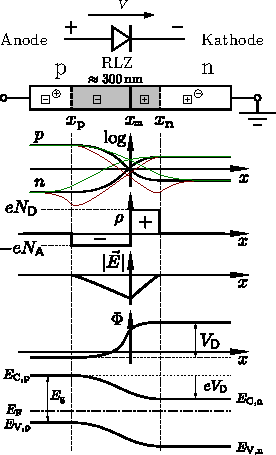
\includegraphics[width = 3.5cm]{./img/pn_junction} }
\parbox{3.1cm}{



\textbf{Raumladungszone RLZ:} \\ Ortsfeste Ladungen, keine freie Ladung, weiter in schwacher Dotierung\\ \\
\textbf{Raumladungsdichte} $\rho$ \\ mit gleichen Flächen:\\
$e N_D \Delta x = -e N_A \Delta x$ \\
\\
\textbf{Feldstärke} $\vec E$\\
$\vec E(x) = - \frac{e N_{\ir A}}{\varepsilon} \Delta x$\\


$\frac{\rho}{\varepsilon} = \frac{\diff E}{\diff x}$\\
Durchbruchspannung $V_{\ir Br} = $


Raumladungszonenlänge $l = $\\
Typisch: $l = 0.1 - \SI{150}{\micro\meter}$\\
Raumladungszonenfeld $\vec E = $\\

Mit steigender Temperatur wandert $E_{\ir F}$ zur Bandmitte
}

\subsection{Gleichgewicht}


\subsection{Flusspolung $V > 0$}
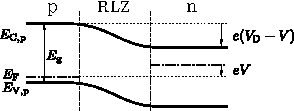
\includegraphics[width = 3.5cm]{./img/pn_voltage.pdf}\\


\subsection{Sperrpolung $V < 0$}
Durchbruchsmechanismen:\\
\begin{itemize}
	\item Thermischer Durchbruch (irreversibel)
	\item Zenereffekt (reversibel): Tunneln $T \upa \Ra V_{\ir Br} \downa$
	\item Lawinendurchbruch (reversibel) $\vec E$-Feld Beschleunigung\\ Dotierung $\upa \Ra \vec E_{\ir RLZ} \upa \Ra V_{\ir Br} \downa$
\end{itemize}

\subsection{Ladungsträgerspeicherung in der RLZ}
Sperrschichtkapazität: Majoritätsträgerspeicherung\\
Diffusionskapazität: Minoritätsträgerspeicherung\\


\subsection{Schottky-Diode}
Schleusenspannung $0.3 \ldots 0.4 V$\\
Schnelle Schaltzeiten


\subsection{Photodiode}
Durch ein Photon generiertes $e/h$-Paar wird durch das el. Feld in der RLZ sofort getrennt.\\
$I_{\ir L} = e \cdot \frac{P_{\ir L}}{E_{\ir Ph}} \cdot \eta_Q(\lambda) = e \cdot \frac{P_{\ir L} \lambda}{h c} \eta_Q(\lambda)$\\
Quantenwirkungsgrad $\eta_Q(\lambda) \in [0,1]$ wie viele Photonen umgewandelt werden\\
Grenzwellenlänge $\lambda_{\ir g}$ minimale Energie um ein Elektron vom Valenzband ins Leitungsband zu heben.\\
Photonen die zu $L_{ir L}$ beitragen: RLZ + Diffusionsgebiete\\
Verdopllung der Leistung: $I_{\ir KS}' = 2 I_{\ir KS}$ \quad $U_{\ir LL}' = U_{\ir LL} + U_{\ir T} \ln(2)$

Wellenlängen, Farbe, Bandabstand\\
% Tabelle der wichtigsten Halbleiter: Bandlücke, Gitterabstand, Effekt Masse
\begin{tabular}{ll}
grün & InN,GaP\\
gelb & InN\\
UV & GaN\\
blau & InGaN\\
\end{tabular}

}
% =========================================================================



\subsection{pin-Diode}
Wird zur Signalübertragung genutzt und mit Sperrspannung betrieben.\\
$p$-Gebiet, intr. Gebiet, $n$-Gebiet\\ 







% SECTION =================================================================
\section{Verständnis}
% =========================================================================
\sectionbox{
	
	\subsection{Größenordnungen für Si:}
	\begin{tabular}{ll}
		Atomedichte & $\SI{e22}{\per\centi\meter^3}$\\
		Eigeneleitungsdichte & $\SI{e10}{\per\centi\meter^3}$\\
		Schwache Dotierung & $\SI{e12}{\per\centi\meter^3}$\\
		Mittlerer Dotierung & $\SI{e15}{\per\centi\meter^3}$\\
		Starke Dotierung & $\SI{e18}{\per\centi\meter^3}$\\
	\end{tabular}	
}
% =========================================================================





% SECTION =================================================================
\section{Bipolartransistor (Analogtechnik)}
% =========================================================================
\symbolbox{
	\begin{tabular}{llll}
	Basisweite $W$ & Diffusionslänge $L$\\
	\end{tabular}
}
Stromverstärker!\\

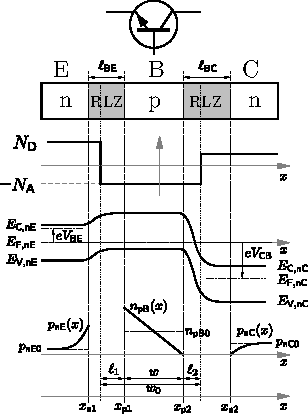
\includegraphics{./img/bipolartransistor.pdf}



\sectionbox{
\subsection{Arten}
NPN und PNP

}

\sectionbox{
\subsection{Verschaltung}
\begin{tabular}{lll}
Basisschaltung & Kollektorschaltung & Emitterschaltung\\
--- Bild --- & --- Bild --- & --- Bild ---\\

\end{tabular}

}

\subsection{Kennlinie}
Early-Effekt: Sättigungslinien schneiden sich im negativen in einem Punkt!\\
$V_{\ir BC} \upa \Ra \ell_{RLZ,CB} \upa \Ra w \downa \Ra \grad(n_{\ir B}(x)) \upa \Ra I_{\ir CE} \upa$

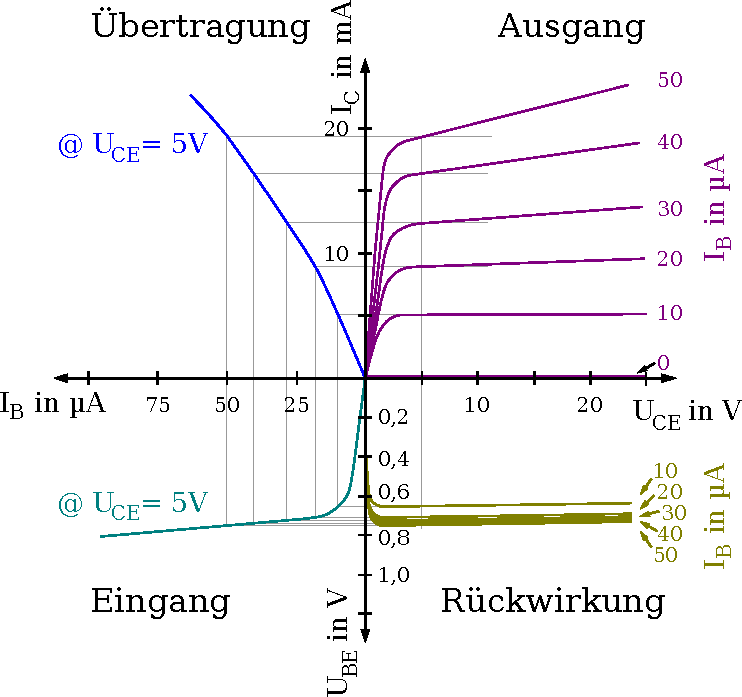
\includegraphics[width = \columnwidth]{./img/bpt_kennlinie.pdf}

Aktiver Bereich: EB-Diode in Fluss, BC-Diode gesperrt\\
Sättigung: beide pn-Übergänge in Flussrichtung\\


\subsection{Basisstrom}
$I_{\ir B} = I_{\ir BE} + I_{\ir BB} + I_{\ir BC}$\\
$I_{\ir BE}$: Löcherinjektion von Basis $\ra$ Emitter\\
$I_{\ir BB}$: Rekombination\\
$I_{\ir BC}$: Löcher absaugen von Kollektor, sehr gering\\



% SECTION =================================================================
\section{Metal-Oxide-Semiconductor-Fiel-Effekt-Transistor MOSFET (Digitaltechnik)}
% =========================================================================
Substrat entgegengesetz zum Kanal: $n$-Substrat $\Ra$ $p$-Kanal MOSFET\\
Gate dotierung verändert nur Einsatzspannung!\\
Inversionspunkt: Eigenleitungsenergie $E_{\ir i}$ und Fermienergie $E_{\ir F}$ ist gleich.\\


Drainstromformel:\\

\subsection{Durchbruchsmechanismen}
\begin{itemize}
	\item Gate-Durchbruch: Zerstörung des Oxids
	\item Source-Drain-Durchbruch:\\
		Punchthrough: Berührung der RLZs\\
		Lawinendurchbruch: Hohes Feld, Stoßionisation
	\item Degradation: Oxidstrom bei Sättigung
\end{itemize}

\subsection{Betriebszustände}
\begin{description}
	\item[Akkumulation:] keine RLZ, $V_{\ir G} < V_{\ir FB} < 0$\\
		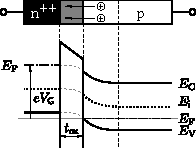
\includegraphics{./img/mos_accumulation.pdf}
	\item[Flachband:] $V_{\ir G} = V_{\ir FB} < 0$\\
		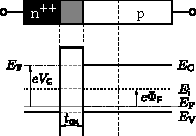
\includegraphics[scale = 0.98]{./img/mos_flatband.pdf}
	\item[Verarmung:] $V_{\ir G} \ge 0$\\
		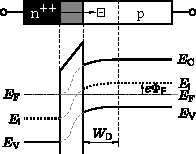
\includegraphics{./img/mos_depletion.pdf}
	\item[Inversion:] $V_{\ir G} \ge V_{\ir T}$\\
		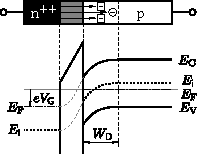
\includegraphics{./img/mos_inversion.pdf}\\
		Starke Inversion: $\Delta E_{\ir i} > 2 e \Phi_{\ir F}$
\end{description}


	\subsection{Transfergate}




% SECTION =================================================================
\section{Halbleiter-Speicher}
% =========================================================================



% SECTION =================================================================
\section{Leistungsbauelemente}
% =========================================================================




% SECTION =================================================================
\section{Grundlagen der Technologie}

Fotodiode: $I_{ph} \propto A$\\
Schottky-Diode: Übergang Metall zu niedrig dotiertem HL\\
Hochdotierung des PN-Übergangs $\Ra$ Schmale Raumladungszone\\


	\subsection{Gewinnung von Silizium}
	
	\begin{enumerate}
		\item Im Hochofen: $\ce{SiO2 + C -> Si + Co2}$\\
			98 \% rein: 1 euro pro Kg
		\item Hochreinigen $\ce{2HCl}$\\
		99,999999999 \% rein
		\item Wafer mit Impfkristall ziehen und polieren
		\item Wafer mit Säure ätzen: Bindung einer einzelne Einheitszelle auf der Oberfläche wird gelöst, glatte verbundene Flächen bleiben unangegriffen
		\item VerbundHL: Aufdampfen oder Molekularstrahlepitaxie 
	\end{enumerate}
	
	
	\subsection{Oxidation}
	Trockene Ox. $\ce{Si + O2 -> SiO2}$ \qquad (langsam)\\
	Feuchte Ox. $\ce{Si + 2H2O -> SiO2 + 2H2}$ \qquad (schnell)\\
	Nitrose Ox. $\ce{Si + 2N2O -> SiO2 + 2N2}$ \qquad (sehr langsam)\\


	\subsection{Lithographie}
	Hauptquelle: Hg-Dampf-Lampe



	\subsection{Dotierung}
	tempern: beim dotieren entstandene Gitterfehler werden durch brownsche Molekularbewegung repariert.



% FUN =====================================================================
% Was sind Halbleiter? Die Maschinenbauer wollen immer was zum anfassen, deswegen mal ich ne Leiter und streich die Hälfte weg.
%
% =========================================================================

% Ende der Spalten
\end{multicols*}

% .:: Dokumentende ======================================================================
\end{document}
